\chapter{Zrýchlenie FSFSOD}\label{chap:proposal}

Ako sme videli v predošlej kapitole fine tuning Frustratingly Simple Few Shot Object Detection~\cite{FSFSODT} trvá pomere dlho a v žiadnom prípade sa nedá použiť v real-time na učenie nových objektov. Preto sa v tejto kapitole pozrieme na to ako by sa dal zrýchliť. 

\section{Zrýchlenie pomocou zmeny parametrov}

Pri pokuse o zrýchlenie fine-tuningu mi ako prvé napadlo zmena trénovacích parametrov. Parametre ktoré majú vplyv na dĺžku tréningu sú batch-size a počet trénovacích iterácii. Pri batch-size sme obmedzený pamäťou našej grafickej karty a maximálny batch size, ktorý zvladne je 2, takže s týmto parametrom nepohneme. Avšak všimol som si, že počas fine-tuningu sa náš model trénuje na začiatku veľmi rýchlo a časom sa veľmi spomaluje. 

Najobjektívnejšiu metriku, ktorú máme počas tréningu je total loss. Vyskúšame ako sa mení počas 1-shot fine-tuningu. Na začiatku má hodnotu 0.7237 a na konci 0.09278. Behom prvej minúty klesne približne na 0.25. Po piatich minútach ma hodnotu 0.17. Po 20 minútach je na hodnote 0.13 a ďalších 35minút veľmi pomaly klesá až na finálnu hodnotu 0.09278. Celý priebeh vidíme na obrázku \ref{fig:image5}.

\begin{figure}[H]
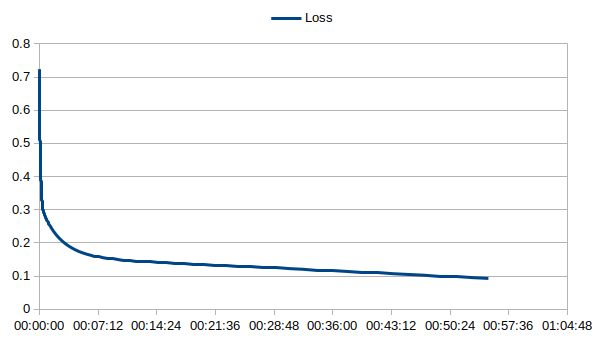
\includegraphics[width=\textwidth]{images/1_shot_training_curve.png}
\centering
\caption{Celková strata počas 1-shot fine tuningu}
\label{fig:image5}
\end{figure}

Už po piatich minútach máme náš model podľa tejto metriky výrazne natrénovaný. Pozrime sa teda na ostatné metriky presnosti po 5 minútach tréningu. Vyskúšame teda najprv znížiť počet iterácií, tak aby tréning trval približne 5 minút a teda znížime počet iterácií z 32 000 na 3 200 a uvidíme ako veľmi nám klesne presnosť pri znížení trénovacieho času o desatinu.

\begin{table}[H]
\begin{tabular}{|l|c|c|c|}
\hline
\textbf{Presnosť} & \textbf{Base} & \textbf{Novel} & \textbf{Priemer} \\
\hline
mAP & 51.505 & 0.114 & 36.822 \\
mAP50 & 78.865 & 0.379 & 56.44 \\
mAP75 & 57.286 & 0 & 40.919 \\
\hline
\end{tabular}
\centering
\caption{Tabuľka presností na testovacích dátach po 5 min. tréningu pre 1-shot detekciu.}
\label{tab:table50}
\end{table}

\begin{figure}[H]
\centering
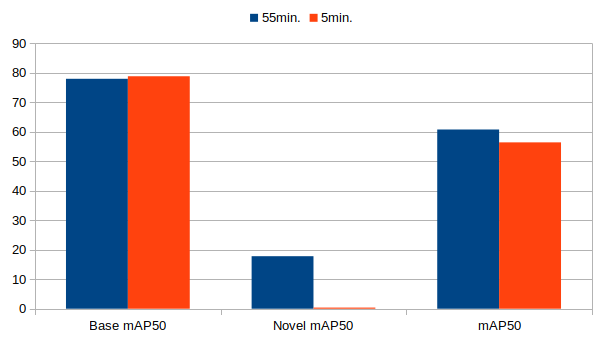
\includegraphics[width=\textwidth]{images/chart_compare_5min.png}
\caption{Porovnanie mAP50 na testovacích dátach 5 min. tréningu s plným tréningom.}
\label{fig:image2}
\end{figure}

Ako vidíme v tabuľke \ref{tab:table50} a na obrázku \ref{fig:image2} priemerná presnosť síce ostala celkom vysoká a presnosť pre base classes je dokonca vyššia, ale pre nás je najdôležitejšia presnosť pre novel classes a tá má veľmi nízke hodnoty, takže takéto skrátenie tréningu nám prinieslo veľmi zlé výsledky. Vyskúšame teda ešte skrátiť tréning na 20 minút a teda znížime počet iterácii z pôvodných 32 000 na 12 000.

\begin{table}[H]
\begin{tabular}{|l|c|c|c|}
\hline
\textbf{Presnosť} & \textbf{Base} & \textbf{Novel} & \textbf{Priemer} \\
\hline
mAP & 50.479 & 4.092 & 37.226 \\
mAP50 & 78.541 & 8.326 & 58.479 \\
mAP75 & 56.248 & 3.701 & 41.235 \\
\hline
\end{tabular}
\centering
\caption{Tabuľka presností na testovacích dátach po 20 min. tréningu pre 1-shot detekciu.}
\label{tab:table51}
\end{table}

\begin{figure}[H]
\centering
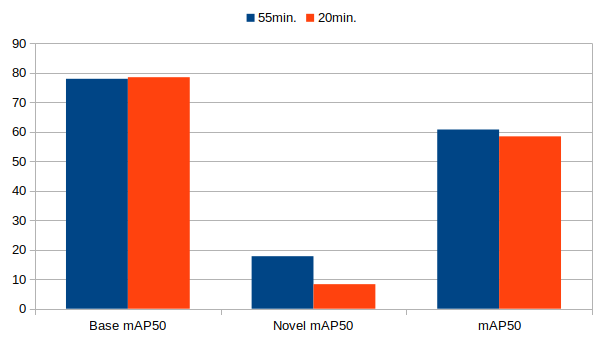
\includegraphics[width=\textwidth]{images/chart_compare_20min.png}
\caption{Porovnanie mAP50 na testovacích dátach 20 min. tréningu s plným tréningom}
\label{fig:image4}
\end{figure}

V tabuľke \ref{tab:table51} vidíme výsledky po 20 minútach a na obrázku \ref{fig:image4} porovnanie presnosti s plným tréningom. Priemerná presnosť sa oproti 5 minútovému tréningu zvýšila len trochu a vidíme taktiež, že sa nám zvýšila presnosť pre novel classes, ale stále je viac ako o polovicu nižšia ako pri plnom čase tréningu.


\section{Zrýchlenie pomocou zapamätania si výstupu zo zmrazených vrstiev}

Predošlý pokus o zrýchlenie nebol veľmi úspešný, avšak zistil som, že počas tréningu prechádza každý batch vždy celou sieťou, napriek tomu, že pri fine tuningu je takmer celá sieť zmrazená okrem poslednej vrstvy (Box Predictor). Vyskúšame teda prejsť zmrazenou časťou siete pre každý vstup len raz a zapamätať si výstup z tejto časti siete pre každý vstup a následne používať len tento predom vypočítaný výstup zo zmrazenej časti siete pre zvyšok tréningu, čo by malo výrazne urýchliť prechod sieťou.

\subsection{Zapamätanie si výstupu z backbone}

Ako sme si popísali v 3. kapitole naša sieť sa skladá z 3 hlavných častí: Backbone, RPN a Roi Heads. Drvivú väčšinu našej siete tvorí Backbone, ktorej výstup ide do RPN a Roi Heads. Do Roi Heads ide taktiež výstup z RPN. V našom prípade pri fine-tuningu sú zmrazené všetky vrstvy okrem poslednej - Box Predictor. Keďže vstupom pre Box Predictor je len výstup z Box Head, potrebujeme si zapamätať výstup z Box Head. Keďže, výstupom Box Predicotra je len zoznam s dvomi hodnotami:  

\begin{enumerate}
  \item Class Prediction: pravdepodobnostné rozloženie medzi triedami objektov
  \item Bounding Box Regression: posun pôvodných súradníc bounding boxu z RPN 
\end{enumerate}

potrebujeme si taktiež zapamätať informácie o návrhoch regiónov, teda výstup z RPN, pre následné vypočítanie straty kvoli tréningu.

Keďže zapamätanie si výstupu pre každý obrázok z Box Head vrstvy, ktorá je súčasťou Roi Heads a výstup návrhov regiónov, ktoré sú výstupom z RPN, je implementačne náročnejšie. Vyskúšame najprv zapametanie si výstupu z Backbone, ktorý aj tak tvori 90\% siete a mal by priniesť výrazné zrýchlenie. Ak by nám to neprinieslo očakávané zrýchlenie, nebude mať zmysel posúvať túto myšlienku ďalej a zapamätávať si výstup priamo z Box Head a RPN pre každý obrázok, čo by malo maximalizovať rýchlosť tréningu.

Keďže, počas tréningu používame batch size veľkosti 2 a obrázky, ktoré sa berú náhodne z tréningovej množiny sú rôznej veľkosti a taktiež sú niekoľko krát resizované, tak aby bol zachovaný pomer strán. Tieto dva vybrané obrázky sú prispôsobené na rovnakú veľkosť pomocou paddingu aby mohli byť reprezentované v jednom tenzore, pred tým ako prejdu Backbonom. 

Týmto sa nám zapamätávanie výstupov veľmi komplikuje, pretože to aký padding bude pridaný na obrázok zavisí od rozmeru obrázka s ktorým je v batchi. A na to aby sme boli presný museli by sme si pamätať výstup pre každú dvojicu obrázkov zvlášť a to určite nechceme, keďže už pri 1-shot detekcii pri 21 triedach máme 21 obrázkov a každý je 11x resizovaný, čiže 231 obrázkov, teda 231x230 = 53 130 rôznych dvojíc obrázkov a rôznych príznakových máp. 

Máme niekoľko možností ako to riešiť, vyskúšame si každú z nich: 

\subsubsection{1. Padding pre všetky obrázky na rovnakú veľkosť}

Môžme zistiť aké rozmery má najväčší batch a nastaviť padding pre každý obrázok na tieto rozmery. Všetky obrázky by tak mali rovnaký rozmer a taktiež aj ich príznaková mapa. Čiže by sme mohli vyrátať príznakovú mapu pre každý obrázok vo všetkych veľkostiach a jednoducho by sme potom takéto dve príznakové mapy spojili do batchu. Problém je v tom, že obrázky budú obsahovať zbytočne veľa paddingu, a všetky obrázky budú príliš veľke, čo taktiež veľmi spomalí náš tréning. Pri vyskúšaní tohto postupu som zistil, že tieto veľké obrázky zaberali príliš pamäte a nestačila na to ani moja grafická karta.

\subsubsection{2. Prispôsobiť všetky obrázky na rovnakú veľkosť}

Ďalší spôsob, je nastaviť všetkým obrázkom rovnakú veľkosť a to spôsobom, že im nastavím veľkosť dlhšej hrany na veľkosť 480, kratšia hrana sa prispôsobí aby sa zachoval pomer strán a následne je obrázok doplnený paddingom tak aby mal rozmer 480x480.

\begin{table}[ht]
\begin{tabular}{|l|c|c|c|}
\hline
\textbf{Presnosť} & \textbf{Base} & \textbf{Novel} & \textbf{Priemer} \\
\hline
mAP & 4.882 & 0.788 & 3.712 \\
mAP50 & 8.875 & 1.6 & 6.797 \\
mAP75 & 4.684 & 0.874 & 3.596 \\
\hline
\end{tabular}
\centering
\caption{Tabuľka presností na testovacích dátach pre prispôsobené obrázky na rovnakú veľkosť pri uložení výstupu z Backbone pri 1-shot detekcii.}
\label{tab:table52}
\end{table}

\begin{figure}[H]
\centering
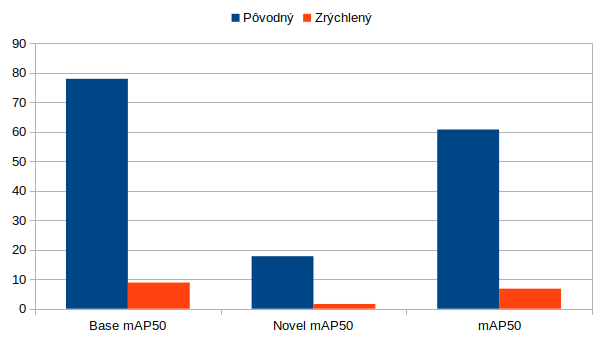
\includegraphics[width=\textwidth]{images/same_size_compare_graph.png}
\caption{Porovnanie presností pôvodného a zrýchleného algoritmu pomocou zapamätania výstupu z Backbone a prispôsobenia obrázkov na rovnakú veľkosť}
\label{fig:image0}
\end{figure}

Tréning sa nám síce podarilo výrazne zrýchliť, trval len 13 minút a 27 sekúnd, avšak ako vidíme v tabuľke \ref{tab:table52} a na obrázku \ref{fig:image0} v porovnaní s presnosťou pôvodného algoritmu naša presnosť veľmi klesla. 

Takúto nízku presnosť máme hlavne preto, že náš model je testovaný na obrázkoch s veľkosťou dlhšej hrany rovnej 800. Skúsili sme teda zmeniť veľkosť testovacích obrázkov na veľkosť dlhšej hrany rovnej 480. Dosiahli sme tak podobné výsledky ako pri pôvodnom tréningu, avšak tento výsledok nie je dostatočne dôveryhodný keďže sme si prispôsobili veľkosť testovacích obrázkov ako sme potrebovali a pri reálnom používaní by bol model menej presný. 

\subsubsection{3. Použiť batch size = 1}

Doteraz sme robili tréning pri batch size veľkosti 2, vyskúšame ako bude algoritmus fungovať pri batch size 1. Ak bude dosahovať dobré výsledky, môže nám to uľahčiť zrýchlenie tréningu. Otestujeme to na 1-shot fine-tuningu, pretože prebieha najrýchlejšie. Prispôsobíme teda trénovacie parametre batch size zmenšíme o polovicu na 1, learning rate taktiež znížime o polovicu z 0.000125 na 0.0000625, zdvojnásobime krok z 24 000 na 48 000 a taktiež zdvojnásobime počet iterácií na 64 000.

\begin{figure}[H]
\centering
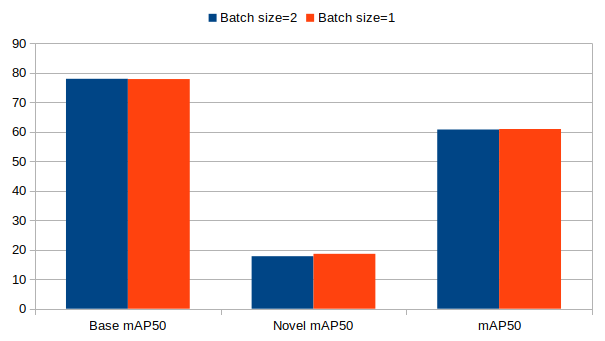
\includegraphics[width=\textwidth]{images/batch_size_comparison.png}
\caption{Porovnanie presnosti pri batch size = 1 a batch size = 2´}
\label{fig:image9}
\end{figure}

Na obrázku \ref{fig:image9} vidíme, že tréning pri batch size veľkosti 1 dosahuje veľmi podobné výsledky ako pri tréningu s batch size 2, avšak tréning bol menej stabilný a celková strata (total loss) počas tréningu s batch size 1 skákala z iterácie na iteráciu s oveľa väčším rozptylom. Čo môže spôsobiť rozptyl vo výsledkoch pri viacerých tréningoch. Každý tréning sa môže podariť inak a pri batch size 1 máme nižšiu konzistenciu. 

Toto sa nám ale podarilo vyriešiť pomocou zmeny Checkpointera. Checkpointer zaznamená aktuálny stav modelu a uloží ho do súboru. Predtým sme používali PeriodicCheckpointer, ktorý vytvoril checkpoint periodicky po rovnakom počte iterácií. Počet iterácii po ktorých sa spraví checkpoint je nastaviteľný a mali sme ho nastavený na 500. Použijeme však BestCheckpointer, ktorý spraví checkpoint ak bola total loss nižšia v aktuálnej iterácii ako v poslednom checkpointe. Nastavíme ho aby kontroloval každých 100 iterácií. Následne ako finálny model berieme posledný checkpoint. 

Tento tréning s batch size 1 trval dokonca o 4 minúty kratšie. Zrejmä preto, že spojiť 2 obrázky rôznych rozmerov do jedneho batchu je výpočtovo náročnejšie. A keďže osahuje veľmi dobré výsledky, stojí za to ho využiť v tomto princípe. 

\subsubsection{1.pokus}

Vyskúšame si teda zapamätať výstup z Backbone pre každý obrázok a následne už Backbonom prechádzať nebudeme. Uvidíme ako to zrýchly náš tréning a aký výsledok dosiahneme. 

Čas nášho tréningu výrazne klesol, tréning trval iba 20 min. oproti pôvodným 55 min. Avšak taktiež klesla naša presnosť ako vidíme na obrázku \ref{fig:image11} v porovnaní s pôvodným tréningom. Hlavným dôvodom poklesu presnosti bude vynechávanie augmentácií počas tréningu, keďže pre každý obrázok si zapamätáme príznaky iba pre jednu transformáciu toho obrázku. Pôvodne počas sa počas tréningu aplikovali na obrázok rôzne augmentáciu a to zmena veľkosti a taktiež náhodné horizontálne otočenie. 

\begin{table}[H]
\begin{tabular}{|l|c|c|c|}
\hline
\textbf{Presnosť} & \textbf{Base} & \textbf{Novel} & \textbf{Priemer} \\
\hline
mAP & 41.895 & 1.52 & 30.359 \\
mAP50 & 74.852 & 5.143 & 54.935 \\
mAP75 & 41.896 & 0.347 & 30.025 \\
\hline
\end{tabular}
\centering
\caption{Tabuľka presností na testovacích dátach 1. pokusu o zrýchlenie pri batch size = 1.}
\label{tab:table53}
\end{table}

\begin{figure}[H]
\centering
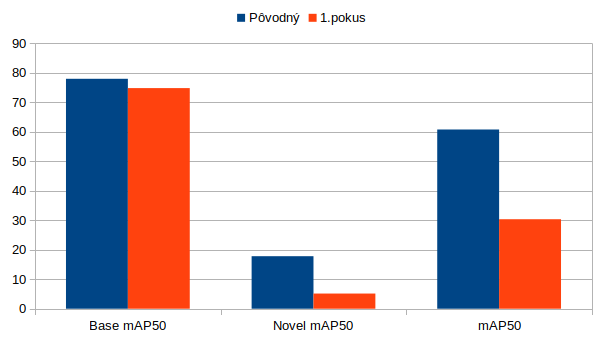
\includegraphics[width=\textwidth]{images/faster_1attempt_chart.png}
\caption{Graf porovnania mAP50 na testovacích dátach pôvodného algoritmu a 1. pokusu o zrýchlenie pri batch size = 1.}
\label{fig:image11}
\end{figure}

\subsubsection{2.pokus}
Pre zvýšenie našej presnosti si vyskúšame zapamätať každý obrázok vo všetkých jeho šírkach. Pokúsime naše príznaky pre každý obrázok v každej veľkosti zapísať do súboru a následne čítať počas tréningu z neho. Po zapísaní príznakov každého obrázku pre všetky veľkosti do súboru bez náhodného horizontálneho otočenia, náš tréning trval približne 33 minút. Dosiahli sme ale požadované rovnaké výsledky ako pri pôvodnom 55 minútovom tréningu, dokonca o trochu lepšie. Podarilo sa nám teda zrýchliť tréning takmer o polovicu. V tabuľke \ref{tab:table55} vidíme výsledky tréningu a na obrázku \ref{fig:image15} porovnanie s pôvodným tréningom. 

\begin{table}[H]
\begin{tabular}{|l|c|c|c|}
\hline
\textbf{Presnosť} & \textbf{Base} & \textbf{Novel} & \textbf{Priemer} \\
\hline
mAP & 49.184 & 10.262 & 38.064 \\
mAP50 & 77.915 & 19.747 & 61.296 \\
mAP75 & 54.58 & 9.522 & 41.707 \\
\hline
\end{tabular}
\centering
\caption{Tabuľka presností na testovacích dátach 2. pokusu o zrýchlenie pri batch size = 1.}
\label{tab:table55}
\end{table}

\begin{figure}[H]
\centering
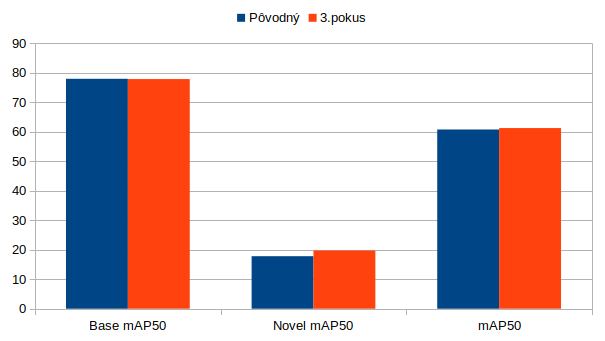
\includegraphics[width=\textwidth]{images/faster_3attempt_chart.png}
\caption{Graf porovnania mAP50 na testovacích dátach pôvodného algoritmu a 2. pokusu o zrýchlenie pri batch size = 1.}
\label{fig:image15}
\end{figure}

\subsection{Zapamätanie si výstupu priamo z Box Head}

Ako sme videli v predošlej časti, uloženie výstupov z Backbone vrstvy do súborov, pre každý obrázok a pre každú veľkosť zvlášť, nám urýchlilo náš tréning takmer o dvojnásobok a zachovala sa naša presnosť. Pokúsime sa teda tréning ešte zrýchliť uložením si výstupov priamo z Box Head a RPN, keďže tieto dva výstupy sú vstupom pre Box Predictor (posledná vrstva ktorú chceme trénovať).To by malo následne vo zvyšku tréningu výpočtovú zložitosť znížiť a ešte zrýchliť náš tréning. Uvidíme ako veľmi to zrýchli náš tréning v porovnaní z predošlím tréningom. 

\begin{table}[H]
\begin{tabular}{|l|c|c|c|}
\hline
\textbf{Presnosť} & \textbf{Base} & \textbf{Novel} & \textbf{Priemer} \\
\hline
mAP & 49.345 & 10.218 & 38.166 \\
mAP50 & 78.011 & 20.032 & 61.446 \\
mAP75 & 54.54 & 9.401 & 41.643 \\
\hline
\end{tabular}
\centering
\caption{Tabuľka presností na testovacích dátach finálneho zrýchleného algoritmu.}
\label{tab:table56}
\end{table}

\begin{figure}[H]
\centering
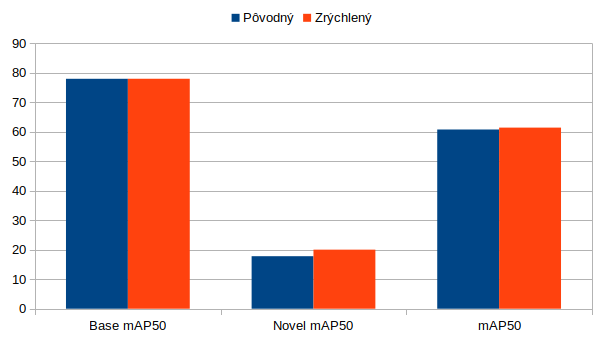
\includegraphics[width=\textwidth]{images/fastest_chart.png}
\caption{Graf porovnania mAP50 na testovacích dátach pôvodného a zrýchleného algoritmu.}
\label{fig:image17}
\end{figure}

V tabuľke \ref{tab:table56} vidíme výsledky nášho pokusu a na obrázku \ref{fig:image17} vidíme porovnanie s pôvodným pomalým algoritmom. Vidíme, že sa nám podarila dosiahnuť rovnaká presnosť. A vyrazne sa nám podarilo zrýchliť tréning celkový čas tréningu bol 6 minút a 51 sekúnd, čo je je takmer 8x rýchlejšie ako pôvodný tréning.

\subsubsection{Riešenie pre rôzne batch size}

Podarilo sa nám náš tréning výrazne zrýchliť, avšak s obmedzením na trénovanie s batch size = 1. Problém s väčším batchom bol ten, že obrázky, ktoré boli spolu v batchi s rôznou veľkosťou a pomerom strán, tak k menšiemu obrázku bol pridaný padding, aby spolu rozmerovo sedeli a keď som si zapamätal príznaky pre ten obrázok s paddingom, keď bol následne v batchi s menším obrázkom a nebol mu pridaný žiadny padding jeho rozmer sa líšil a musel som si zapamätať výstup aj pre tento rozmer. A teda pri väčšej batch size som si musel pamätať výstupy z Box Head a RPN pre každý obrázok v každom jeho rozmere v ktorom sa objavil v batchi a teda oveľa viac dát, čo spôsobovalo veľmi vysokú pamäťovú náročnosť. Tento problém už však nemáme, keďže výstupy z vrstiev si ukladáme do súborov na disk.

Po upravení implementácie aby fungoval náš algoritmus pre rôzne batch size, sme schopný trénovať na rôznych batch size na našom GPU, dokonca aj vyššie hodnoty ako napríklad 16, keďže náš algoritmus ukladaním výstupov do textových súborov dosahuje oveľa nižšiu pamäťovú náročnosť pre GPU. Miesto toho aby si pamätal výstupy z jednotlivých vrstiev pre celý batch počas jednej iterácie, si ich nemusí pamätať a načíta si ich zo súboru. A pri ukladaní výstupov to robí postupne pre každý obrázok zvlášť.

Vyskúšame porovnať presnosť a dĺžku 1-shot tréningu pri rôznych batch size s tým, že prispôsobíme počet iterácii a learning rate. Pri zdvojnásobení batch size, zmenšíme počet iterácii na polovicu a zdvojnásobíme learning rate. 

\begin{figure}[H]
\centering
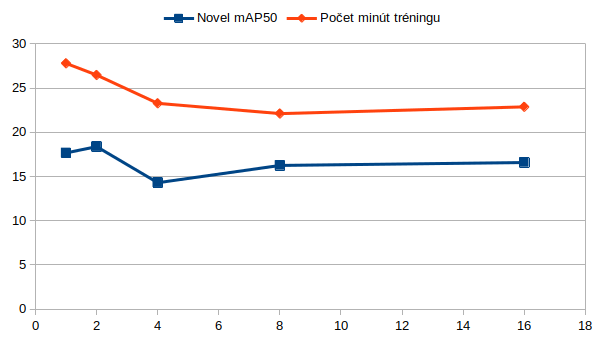
\includegraphics[width=\textwidth]{images/diff_batch_size.png}
\caption{Porovnanie presnosti na testovacích dátach a dĺžky tréningu rôznych batch size.}
\label{fig:diff_batch_size}
\end{figure}

Na obrázku \ref{fig:diff_batch_size} vidíme porovnanie novel mAP50 a dĺžky tréningu pri rôznych batch size. Vidíme, že čas tréningu je veľmi podobný a najvyššiu presnosť dosahujeme pri batch size = 2. Pri tomto pokuse sme použili iné náhodné obrázky na tréning, takže presnosť novel mAP50 sa trochu líši od predošlých pokusov. 


\subsubsection{Vyhodnotenie}

\begin{figure}[H]
\centering
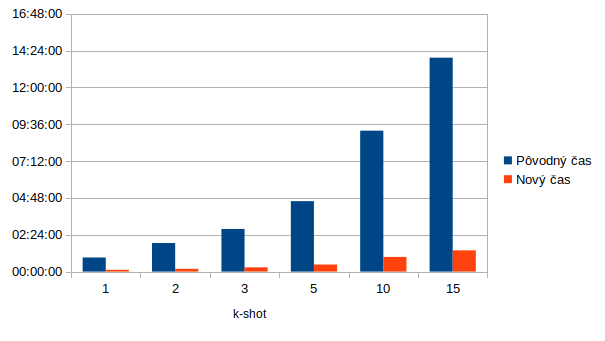
\includegraphics[width=\textwidth]{images/speed_compare.png}
\caption{Porovnanie rýchlostí pôvodného algoritmu a algoritmu po zrýchlení}
\label{fig:image500}
\end{figure}

Na obrázku \ref{fig:image500} vidíme porovnanie rýchlosti pôvodného algoritmu a algoritmu po zrýchlení pri rôznych k-shot tréningoch. Oba algoritmy dosahujú podobnú presnosť.






